\documentclass[fleqn,10pt]{wlscirep}
\title{Assessing heterogeneity (and predictability ??) of runners' performance in Switzerland}

\author[1,*]{Gianrocco Lazzari}
\author[2]{Stefano Savaré}
\author[2]{Antonio Iubatti}
\author[2]{Maxime Peschard}
\author[2]{Ondine Chanon}
\author[2]{Michele Catasta}
\author[1]{Marcel Salathé}
\affil[1]{1. Global Health Institute, School of Life Sciences, Ecole Polytechnique Fédérale de Lausanne (EPFL), Lausanne, Switzerland.}
\affil[2]{2. School of Computer Science, Ecole Polytechnique Fédérale de Lausanne (EPFL), Lausanne, Switzerland.}

\affil[*]{gianrocco.lazzari@epfl.ch}

%\affil[+]{these authors contributed equally to this work}

%\keywords{Aging, Distance running, Endurance performance, Sex difference}

%%%% %%%% %%%% %%%%  GR's packages %%%% %%%% %%%% %%%% %%%% 

\usepackage{caption,subfigure,float}
%\usepackage{subcaption} 

% for an examples please fer to http://tex.stackexchange.com/questions/148438/putting-two-images-beside-each-other

%packages for references
\usepackage{hyperref,url,cite}


%%%% %%%% %%%% %%%% %%%% %%%% %%%% %%%% %%%% %%%% %%%% %%%% 

\begin{abstract}
	
%Example Abstract. Abstract must be under 200 words and not include subheadings or citations. 



	\textbf{keywords}: Aging, Distance running, Endurance performance, Sex difference

\end{abstract}
\begin{document}

\flushbottom
\maketitle
% * <john.hammersley@gmail.com> 2015-02-09T12:07:31.197Z:
%
%  Click the title above to edit the author information and abstract
%
\thispagestyle{empty}

%\noindent Please note: Abbreviations should be introduced at the first mention in the main text – no abbreviations lists. Suggested structure of main text (not enforced) is provided below.

\section*{Introduction}

%The Introduction section, of referenced text\cite{Figueredo:2009dg} expands on the background of the work (some overlap with the Abstract is acceptable). The introduction should not include subheadings.

as show in \cite{connick2015relative} blabalblab 

\section*{Results}

%Up to three levels of \textbf{subheading} are permitted. Subheadings should not be numbered.
%
%\subsection*{Subsection}
%
%Example text under a subsection. Bulleted lists may be used where appropriate, e.g.
%
%\begin{itemize}
%\item First item
%\item Second item
%\end{itemize}
%
%\subsubsection*{Third-level section}
% 
%Topical subheadings are allowed.

	\subsection*{Demographics}
	
		In fig. \ref{participation_overall_by_distance} and \ref{participation_overall_by_gender} we show respectively how number of runners increased in the last 15 years, by distances and gender. This raise was faster for man then for women, and faster in the shorter distances (10 Km) than for longer one (participants in full marathons, 42 Km, seems to have decreased) \footnote{For simplicity we only include th e most popular distances. There are many events that include shorter distances, like 3 Km, 5 Km, usually attended by few young runners.}.
		
		
				\begin{figure*}[h]	
			
					\centering
					
					\subfigure[]{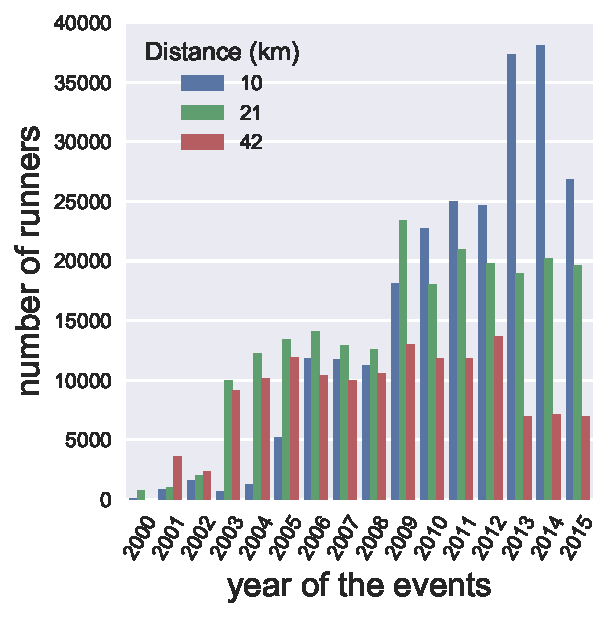
\includegraphics[scale=0.8]{../data_analysis/plots_for_paper/participation_overall_by_distance.pdf}\label{participation_overall_by_distance}}
%					\hfill
					\subfigure[]{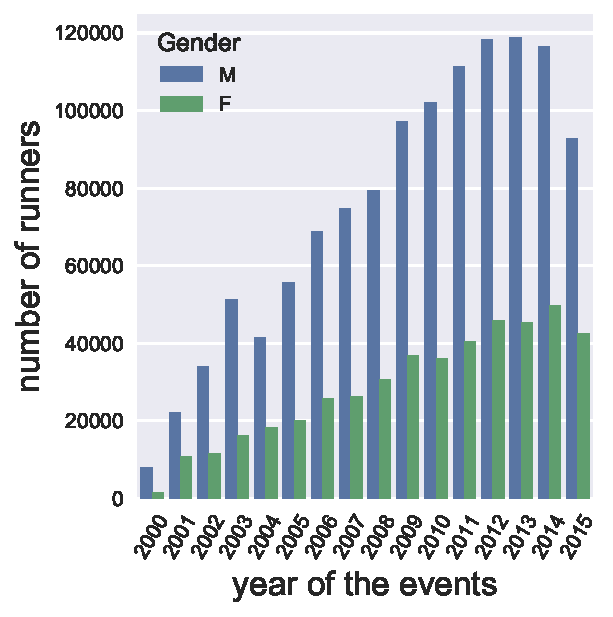
\includegraphics[scale=0.8]{../data_analysis/plots_for_paper/participation_overall_by_gender.pdf}\label{participation_overall_by_gender}}
					
					\caption{Number of participants in running competition in Switzerland, across time, by distance and gender.}
					
			
		\end{figure*}		
	
			
	\subsection*{The case of Lausanne Marathon}
		
	

	\subsection*{Overall performance analysis}
	
		\subsubsection*{Age-performance relation}
		
			remember to cite the relevant papers 
			\cite{knechtle2014relationship}
			\cite{connick2015relative}
			\cite{lara2014relationship}
			\cite{lehto2016effects}
			
		\subsubsection*{Temperature-performance relation}
		
			we don't have enough data (can be re-checked)...\\
			
			some reviews on the topic:\\
			\url{http://runningstrong.com/temperature.html}\\
			\url{http://believeperform.com/performance/the-effects-of-heat-on-sport-performance/}
			
	
	
	\subsection*{Geographical analysis}
	
		(to be included ??)
		(by antonio)
	
	
	\subsection*{Network of runners}
	
				(to be included ??)
				(by Gr)
		
	\subsection*{Forecast of career advancement (??)}
	
				(not done yet)		\\
				\href{https://fivethirtyeight.com/features/tell-us-two-things-and-well-tell-you-how-fast-youd-run-a-marathon/}{nice article on fivethertyeight},
				pointing to one of the best/latest model \cite{vickers2016empirical}

	

\section*{Discussion}

%The Discussion should be succinct and must not contain subheadings.

\section*{Methods}

%Topical subheadings are allowed. Authors must ensure that their Methods section includes adequate experimental and characterization data necessary for others in the field to reproduce their work.

	\subsection*{Data parsing}
	
		@stefano
	
		
	
	
	\subsection*{Data analysis}
	
		All analysis were performed on python notebooks (available on the \href{related repository}{related repository}), using standard python packages for data analysis and plotting, such as \texttt{pandas}, \texttt{seaborn}, \texttt{scipy}, \texttt{powerlaw}\footnote{\url{https://pypi.python.org/pypi/powerlaw}} and \texttt{networkx}.
	
	
	\subsection*{Data visualization}		
	
		We implemented interactive visualizations of some of our results and collected  them in the   \href{https://hopsuisse.github.io}{Hop Suisse}\footnote{\url{https://hopsuisse.github.io}} website.
		After exporting the data needed for the plot in \texttt{.json} dumps, we used \href{http://c3js.org}{C3.js} for the interactive plotting. More details on how datasets queries and plots were built can be found on the dedicated \href{https://github.com/hopsuisse/hopsuisse.github.io}{GitHub repository}\footnote{\url{https://github.com/hopsuisse/hopsuisse.github.io}}.
		We also build an \href{https://www.youtube.com/watch?v=MyvbnOXHShw}{animated infographics}\footnote{\url{https://www.youtube.com/watch?v=MyvbnOXHShw}}, inspired by  \href{https://en.wikipedia.org/wiki/Hans_Rosling}{Hans Rosling}'s work. With such video we wanted to show in a more powerful and clear way the relations among runners' mean pace, experience and age, providing as well information on gender and race length
		(the python code used to construct the video frames can be found in the \href{https://github.com/ggrrll/hop_suisse_ada_project_public/tree/master/8-video}{related folder}\footnote{\url{https://github.com/ggrrll/hop_suisse_ada_project_public/tree/master/8-video}} of our GitHub repository).
	
\bibliography{bib_hop_suisse}

%\noindent LaTeX formats citations and references automatically using the bibliography records in your .bib file, which you can edit via the project menu. Use the cite command for an inline citation, e.g.  \cite{Figueredo:2009dg}.

%\section*{Acknowledgements (not compulsory)}
%
%Acknowledgements should be brief, and should not include thanks to anonymous referees and editors, or effusive comments. Grant or contribution numbers may be acknowledged.

\section*{Author contributions statement}

G.L. and A.I. performed the data analysis.
S.S., O.C. and M.P. performed the data parsing.
G.L. and S.S. wrote the manuscript.
M.C. and M.S. review the manuscript.
%M.C. supervised the study.

\section*{Additional information}

All the code used to parse the data from \url{https://www.datasport.com/en/}, for data analysis and visualization can be found in our open GitHub repository: \url{https://github.com/ggrrll/hop_suisse_ada_project_public}.\\

\section*{Competing financial interests}

The authors declare no conflict of interests.

%To include, in this order: 
%\textbf{Accession codes} (where applicable); 
%\textbf{Competing financial interests} (mandatory statement). 
%
%The corresponding author is responsible for submitting a \href{http://www.nature.com/srep/policies/index.html#competing}{competing financial interests statement} on behalf of all authors of the paper. This statement must be included in the submitted article file.

%\begin{figure}[ht]
%\centering
%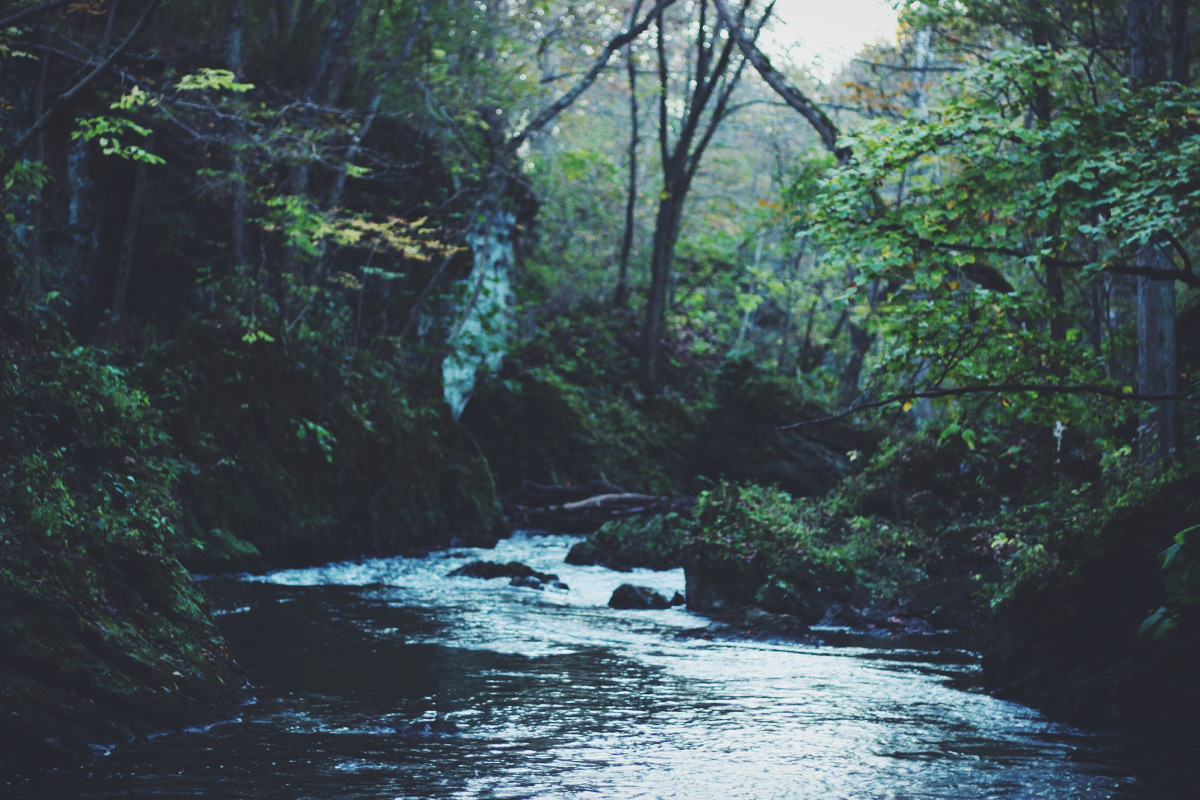
\includegraphics[width=\linewidth]{stream}
%\caption{Legend (350 words max). Example legend text.}
%\label{fig:stream}
%\end{figure}
%
%\begin{table}[ht]
%\centering
%\begin{tabular}{|l|l|l|}
%\hline
%Condition & n & p \\
%\hline
%A & 5 & 0.1 \\
%\hline
%B & 10 & 0.01 \\
%\hline
%\end{tabular}
%\caption{\label{tab:example}Legend (350 words max). Example legend text.}
%\end{table}

%Figures and tables can be referenced in LaTeX using the ref command, e.g. Figure \ref{fig:stream} and Table \ref{tab:example}.

\end{document}